\documentclass[a4paper,14pt]{extarticle}
\usepackage{graphicx}
\usepackage{ucs}
\usepackage[utf8x]{inputenc}
\usepackage[russian]{babel}
\usepackage{multirow}
\usepackage{mathtext}
\usepackage[T2A]{fontenc}
\usepackage{titlesec}
\usepackage{float}
\usepackage{empheq}
\usepackage{amsfonts}
\usepackage{amsmath}
\title{\textbf{Лабораторная работа по взятию производной }}\author{Чурсин Владимир Б01-305}
\begin{document}
\maketitle
\section{\ Производная Функции \\}\begin{center}$f\left(x\right) = x^2+2 \cdot x$ \end{center}\  
\subsection{Решение}\ \newlineОчевидно, что: \\ 

\begin{center}$\left(2 \cdot x \right)' = 2$\end{center}\ 
При этом f(x) и g(x) могут вести себя как угодно: \\ 

\begin{center}$\left(x^2 \right)' = 2 \cdot x$\end{center}\ 
Необходимо сделать предостережение о неверном применении правила Лопиталя: \\ 

\begin{center}$\left(x^2+2 \cdot x \right)' = 2 \cdot x+2$\end{center}\ 
\subsection{Ответ}\ \newlineВ результате получаем: \\
\begin{center}$\left(x^2+2 \cdot x \right)' = 2 \cdot x+2$\end{center}\ 
\section{Разложение по Тейлору}\begin{center}$f\left(x\right) = x^2+2 \cdot x$ \end{center}\ 
\subsection{Решение}\ \newlineТеперь докажем теорему 4.17 из приложения 2.18 по определению 2.18.28: \\ 

\begin{center}$f^{\left(0\right)} = x^2+2 \cdot x$\end{center}\ 
\begin{center}$f^{\left(0\right)}\left(0\right) = 0
$\end{center}\ \newline \\ 
Аналогично определению 4.3 кривой на плоскости дается определение: \\ 

\begin{center}$f^{\left(1\right)} = 2 \cdot x+2$\end{center}\ 
\begin{center}$f^{\left(1\right)}\left(0\right) = 2
$\end{center}\ \newline \\ 
В таком виде она может быть рассмотрена, как суперпозиция: \\ 

\begin{center}$f^{\left(2\right)} = 2$\end{center}\ 
\begin{center}$f^{\left(2\right)}\left(0\right) = 2
$\end{center}\ \newline \\ 
Гладкая кривая в любой точке имеет: \\ 

\begin{center}$f^{\left(3\right)} = 0$\end{center}\ 
\begin{center}$f^{\left(3\right)}\left(0\right) = 0
$\end{center}\ \newline \\ 
\subsection{Ответ}\ \newlineВ результате получаем разложение ряда Тейлора в точке 0:\begin{center}$f\left(x\right) = \frac{2}{1} \cdot{(x)^{1}} + \frac{2}{2} \cdot{(x)^{2}} + o(x^{3})$ \end{center}\ 


\section{Построение графика исходной функции}\ Используя данные, полученные в пунктах 1 и 2, получаем график:
\begin{center} 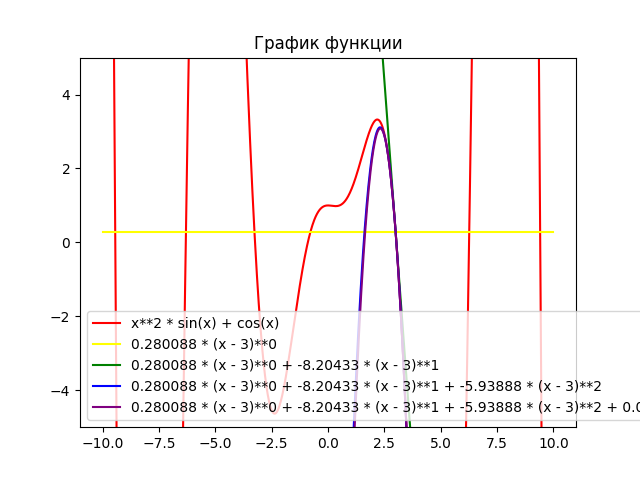
\includegraphics[scale=0.8]{plot.png} \end{center}
\end{document}